\label{sec:NN}
Fully connected or feed-forward neural networks (NNs) also have a long history in high energy physics. The fundamental element of any neural network is called a \textit{layer}. Multiple layers are stacked together to produce a final prediction given the input variables from the first layer. This predicted outcome is then evaluated against a known target value. A fully-connected network can have multiple internal (or hidden) layers between the input and output layers, and each hidden layer is composed of a series of activation functions and trainable weights that allow the network to identify and iteratively combine important features of the input space. A function (called the loss function) is chosen to quantify the difference between the model prediction and target values. The loss calculated after a single training iteration is used to adjust the internal network weights in the next training iteration through a process called backpropagation. The model is fully trained once the improvement in the loss between iterations falls beneath some user-defined threshold.

The NN trained for di-Higgs detection was built using the Keras~\cite{chollet2015keras} and Tensorflow~\cite{tensorflow} packages. The top twenty-two most separable reconstructed and event-level variables were used as the input variables for the NN. These included the mass, momentum, and angular separation variables for the di-Higgs system and the Higgs candidate di-jets, momentum and angular information from the individual selected jets, and all event-level variables. Hyperparameter optimization for neural networks involves the additional step of designing the structure of the network: how many hidden layers to use, how many nodes per hidden layer, which activation functions to use in a given layer, using dropout layers which remove random weights in each training iteration to prevent over-fitting, and adding batch normalization layers which stabilize and accelerate network training by re-scaling the neuron weights of the previous layer.

Several models were trained by individually tuning each hyperparameter over a reasonable range in order to produce a final optimized model. The number of hidden layers was similarly optimized by training models with one, two, three, and four hidden layers. No networks with more than four hidden layers were tested in order to keep the number of trainable model parameters below approximately one tenth the number of training events.

The final network structure consisted of the input layer, two hidden layers, and a single-node output layer. The first hidden layer contained 175 nodes with an L2 kernel regularizer ($\lambda$ = $10^{-4}$). The second hidden layer contained 90 nodes with no kernel regularizer. A batch normalization layer and a dropout layer (dropout fraction 0.2) were placed in between the two hidden layers to prevent over-fitting. Both hidden layers used a rectified linear (ReLU) activation function, while the output layer used a sigmoid activation function. The final performance was found to be independent of the choice of activation functions, and they are included here for completeness. The binary cross-entropy loss function

\begin{equation*}
L = -(y\log(p)+(1-y)\log(1-p))
\end{equation*}
was used for the backpropagation. Here $y$ represents the known binary target classifications, $p$ represents the predicted probabilities that a given event is signal or background, and $\log$ is the natural logarithm. A schematic flowchart of the network structure is shown in Figure~\ref{fig:nn}.
%The sequential model was compiled using the ‘adam’ optimizer along with the ‘binary\_crossentropy’ loss method. Finally, the model was fit on the training data along with the validation data for 100 epochs. 

\begin{figure}[!h] 
\begin{center}
\includegraphics*[width=0.75\textwidth] {ffNN/figures/flowchart_ffNN.png}
\caption{Structure of the feed-forward neural network. The input variables are fed through two fully connected dense layers to classify events. One dropout layer and one batch normalization layer help mitigate over-fitting during training.}
  \label{fig:nn}
\end{center}
\end{figure}

The NN was trained for 25 epochs before the minimal loss-improvement threshold was met, and the results are shown in Figure~\ref{fig:results_nn}. The trained model obtained a maximum $\sigma$ = 2.40$\pm$0.08 when considering events with a signal prediction score > 0.94. This phase-space has a signal yield of $1659.9 \pm 12.5$ events and a background yield of $4.8 \pm 0.2$ $\cdot$ $10^5$ events. %477215.3 events.

\begin{figure}[!h] 
\begin{center}
   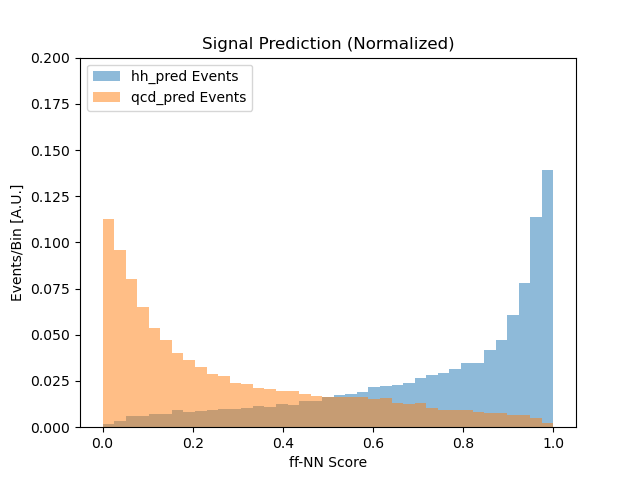
\includegraphics[width = 3in]{ffNN/figures/score_ffnn_v3}\\
\caption{Final predictions of the feed-forward network for signal and background samples.}
  \label{fig:results_nn}
\end{center}
\end{figure}

